% concatenated from main.tex
\documentclass{article}
\usepackage[utf8]{inputenc}
\usepackage{fullpage}

\usepackage{amsmath,amsthm,amssymb}
\usepackage{mathtools}
\usepackage{tikz}
\usepackage{hyperref,cleveref}
\usepackage{todonotes}

\newtheorem{theorem}{Theorem}[section]
\newtheorem{corollary}[theorem]{Corollary}
\newtheorem{lemma}[theorem]{Lemma}
\newtheorem{observation}[theorem]{Observation}
\newtheorem{claim}[theorem]{Claim}
\newtheorem{proposition}[theorem]{Proposition}
\newtheorem{definition}[theorem]{Definition}
\newtheorem{fact}[theorem]{Fact}
\newtheorem{remark}[theorem]{Remark}

\newcommand{\R}{\mathbb{R}}

\usepackage{xspace}
\newcommand{\finalbound}{{\color{orange}187}\xspace}

\begin{document}

\title{Coloring t-perfect graphs with fewer colors}
\author{Matija Novakovi\'c \and Stefan Weltge}
\date{\today}

\maketitle

\begin{abstract}
    Recently, Chudnovsky, Cook, Davies, Oum, and Tan obtained the first finite bound on the chromatic number of t-perfect graphs, showing that they are 199053-colorable.
    We improve this bound to 186 by refining their proof.

    The original proof establishes that every graph with large odd girth and large chromatic number contains a certain structure called an $r$-arithmetic rope, and that its existence in a certain leveling of a graph with large odd girth would imply an odd wheel as a t-minor, a known obstruction of t-perfectness.
    While their technique requires a lower bound on the chromatic number that is exponential in $r$, we show that the existence of an $r$-arithmetic rope can already be guaranteed under a linear bound.
    Using a slightly weakened notion of arithmetic ropes allows us to reduce the bound even further.
\end{abstract}

\section{Introduction}

The stable set problem asks for finding a maximum stable set in a given undirected graph, i.e., a largest set of pairwise non-adjacent vertices.
While the problem is NP-hard in general, it can be solved in polynomial time for several classes of graphs.
A common approach to derive efficient algorithms is to exploit the structure of the \emph{stable set polytope}, which is the convex hull of characteristic vectors of stable sets.
Introduced by Chvátal~\cite{chvatal1975certain}, a prominent example is the class of \emph{t-perfect graphs}, which are defined as the graphs $G$ whose stable set polytope coincides with the set of vectors $x \in [0,1]^{V(G)}$ satisfying $x_u + x_v \le 1$ for every edge $uv \in E(G)$ (edge inequalities) and $\sum_{v \in V(C)} x_v \le \frac12 (|V(C)| - 1)$ for every odd cycle $C$ of $G$ (odd cycle inequalities).

In 1992, Shepherd~\cite[8.14]{jensen2011graph} asked whether the stable set polytope $P$ of a t-perfect graph $G$ always has the integer decomposition property, that is, for every positive integer $k$, every integer point in $kP$ is a sum of $k$ integer vectors points in $P$.
Since the all-$\frac{1}{3}$ vector is contained $P$, this would imply that $G$ is 3-colorable.
In 1994, Laurent and Seymour~\cite[p. 1207]{schrijver2003combinatorial} (and later Benchetrit~\cite{benchetrit2015proprietes,benchetrit20164}) found t-perfect graphs with chromatic number 4, negatively answering Shepherd's question.
Since then, it is an open question whether every t-perfect graph is 4-colorable~\cite[8.14]{jensen2011graph}.

Only recently, Chudnovsky, Cook, Davies, Oum, and Tan~\cite{chudnovsky2024colouringtperfectgraphs} gave the first finite bound on the chromatic number of t-perfect graphs, showing that they are 199053-colorable.
While their proof has not been optimized for the best bound, they expected that carrying out their arguments with more care
\begin{quote}
    ``[...] would still leave a large gap between our bound and the lower bound of 4. A good milestone for narrowing the gap would be to improve our upper bound to at most 1000.''
\end{quote}
We show how their proof can be refined to obtain the following bound.

\begin{theorem}\label{thm:main}
    Every t-perfect graph is 186-colorable.
\end{theorem}

The approach of~\cite{chudnovsky2024colouringtperfectgraphs} is based on only two properties of t-perfect graphs: they do not contain odd wheels as t-minors, and they have a stable set that intersects every shortest odd cycle.
As the main technical contribution, the authors show that every graph with large odd girth and large chromatic number contains a certain structure called an ''arithmetic rope'', and observe that the existence of an arithmetic rope in a certain leveling of a graph with large odd girth would imply the existence of an odd wheel as a t-minor.
We refine their proof and show that the existence of an arithmetic rope can be guaranteed under a much weaker assumption on the chromatic number.
To decrease the bound on the chromatic number even further, we exploit the fact that a slightly weaker structure, which we call a \emph{quasi-arithmetic rope}, is already sufficient for finding an odd wheel t-minor.

\Cref{thm:main} also yields an improved bound on the chromatic number of h-perfect graphs, which are defined as the graphs $G$ whose stable set polytope coincides with the set of vectors $x \in [0,1]^{V(G)}$ satisfying the odd cycle inequalities and $\sum_{v \in Q} x_v \leq 1$ for every clique $Q$ of $G$ (clique inequalities).
Using a result of Sebő (unpublished, see~\cite{bruhn2012claw}) and Marcus~\cite{marcus1996shortestoddcycles}, the authors of~\cite[Thm. 1.2]{chudnovsky2024colouringtperfectgraphs} observe that if every t-perfect graph is $k$-colorable, then every h-perfect graph $G$ is ($\omega(G) + k - 2)$-colorable.
Hence, we obtain the following bound.
\begin{corollary}
    Every h-perfect graph $G$ is $(\omega(G) + 184)$-colorable.
\end{corollary}

In Section~\ref{sec:basics}, we introduce definitions of the aforementioned structures, review the essential steps of the proof of~\cite{chudnovsky2024colouringtperfectgraphs}, describe our main result on the existence of quasi-arithmetic ropes, and explain how this leads to an improved bound on the chromatic number of t-perfect graphs.
The proof of our main result is given in Sections~\ref{sec:quasi_arithmetic_rope}, \ref{sec:segments_odd_and_even}, and \ref{sec:segments_even}.

\section{Quasi-arithmetic ropes and t-minors of odd wheels}
\label{sec:basics}

An essential property of t-perfect graphs is that they are closed under taking t-minors. 
This operation is based on the notion of a \emph{t-contraction}, which refers to the operation of contracting all edges in the closed neighborhood of a vertex whose neighborhood is a stable set.
A \emph{t-minor} of a graph $G$ is a graph obtained from $G$ by a sequence of vertex deletions and t-contractions.
Gerards and Shepherd~\cite{tminorstperfectgerards1998} observed that if $G$ is t-perfect, each of its t-minors is t-perfect as well.

A basic family of graphs that are known not to be t-perfect are the \emph{odd wheels}, which are obtained from odd cycles by adding a new central vertex that is adjacent to all vertices of the cycle.
Consequently, t-perfect graphs do not contain odd wheels as t-minors.

The main contribution of~\cite{chudnovsky2024colouringtperfectgraphs} is to show that graphs with sufficiently large chromatic number and odd girth must contain an odd wheel as a t-minor. Here, the odd girth of a graph is defined as the length of its shortest odd cycle. 
To bound the chromatic number of a t-perfect graph, it is indeed sufficient to consider graphs with large odd girth due to the following fact.

\begin{proposition}[{Marcus~\cite{marcus1996shortestoddcycles}, see also \cite[Lem.~3.4]{chudnovsky2024colouringtperfectgraphs}}]\label{prop:marcus}
    Every t-perfect graph $G$ has a stable set that intersects every shortest odd cycle in $G$.
\end{proposition}

To extract odd wheel t-minors, the authors of~\cite{chudnovsky2024colouringtperfectgraphs} introduce the notion of an arithmetic rope.
We consider the slightly different notion of a \emph{quasi-$r$-arithmetic rope} in a graph $G$, which consists of vertices $q_1,\dots,q_r$ together with paths $Q_{i,1}, Q_{i,2}$ for $i \in [r] = \{1, \dots, r\}$ such that (taking indices modulo $r$)
\begin{itemize}
    \item[a)] each $Q_{i,1}$ and $Q_{i, 2}$ is a $q_iq_{i + 1}$-path,
    \item[b)] each $Q_{i,1}$ has odd length,
    \item[c)] $Q_{i, 2}$ or $Q_{i + 1, 2}$ has even length,
    \item[d)] for every $(h_1,\dots,h_r) \in \{1,2\}^r$, the graph $Q_{1,h_1} \cup \dots \cup Q_{r,h_r}$ is an induced cycle, and
    \item[e)] $q_1, \dots, q_r$ have pairwise $G$-distance at least 6.
\end{itemize}
If all vertices of the paths $Q_{i,1}, Q_{i,2}$ are contained in a vertex set $X \subseteq V(G)$, we say that \emph{$G$ has a quasi-$r$-arithmetic rope in $X$}.
Note that in this case, condition e) still refers to the distance in $G$ and not the distance in $G[X]$.
When constructing quasi-arithmetic ropes, we will make use of the fact that for some $i$, both $Q_{i,1}$ and $Q_{i,2}$ are allowed to have even length.
For notational convenience, we will simply set $Q_{i, 2} = Q_{i, 1}$ in these cases.

Let $N_G^t(u)$ denote the set of vertices with distance exactly $t$ from $u$ in $G$ and let $N_G^t[u] = \bigcup_{i = 0}^t N_G^t(u)$ denote the corresponding closed neighborhood.
A key observation in the proof of~\cite{chudnovsky2024colouringtperfectgraphs} is the following.
\begin{proposition}\label{prop:t_minor_in_rope}
    Let $G$ be a graph with odd girth at least 7, $u \in V(G)$, and $t \ge 4$. If $G$ contains a quasi-$5$-arithmetic rope in $N_G^t(u)$, then $G$ has an odd wheel t-minor.
\end{proposition}
Strictly speaking, the above statement is only shown for arithmetic ropes, which differ from our notion of quasi-arithmetic ropes in the sense that each $Q_{i,2}$ is required to have odd length, and the pairwise $G$-distance between the $q_i$'s to be at least 5. However, their proof only relies on the fact that for every choice of three vertices among $q_1,\dots,q_5$, there is a choice of paths along the $5$-arithmetic rope such that the resulting induced cycle is odd and partitioned into three odd length paths by the three vertices. Since this is also true for our notion of quasi-$5$-arithmetic ropes, their proof directly carries over to our setting, so we refrain from repeating it.

Our main contribution is the following theorem.

\begin{theorem}\label{thm:quasi_rope_existence}
    For $r \in \mathbb{N}$, every graph $G$ with odd girth at least 15 and $X \subseteq V(G)$ contains a quasi-$r$-arithmetic rope in $X$ if 
    \[\chi(X) \geq \begin{cases}
        16r + 5 & \text{if } r \text{ is even,}\\
        16r + 11 & \text{if } r \text{ is odd.}
    \end{cases}\]
\end{theorem}

To see how the above result implies \Cref{thm:main}, assume that $G$ is a t-perfect graph with $\chi(G) \geq 187$. According to \Cref{prop:marcus}, we may iteratively remove six stable sets from $G$ to obtain an induced subgraph $H$ with odd girth at least 15. Note that $\chi(H) \geq 181$. Let $u$ be an arbitrary vertex of a connected component of $H$ with maximum chromatic number and note that there must be a level $t$ with $\chi(N_H^t(u)) \geq \lceil \frac{181}{2} \rceil= 91 = 16\cdot 5 + 11$. Since the odd girth of $H$ is at least 15, $N_H^t[u]$ is bipartite and thus $t \geq 4$. By \Cref{thm:quasi_rope_existence}, $H$ contains a quasi-5-arithmetic rope in $N_H^t(u)$. \Cref{prop:t_minor_in_rope} now implies that $H$ contains an odd wheel t-minor, and so does $G$, contradicting the fact that $G$ is t-perfect.

The authors of~\cite[Thm. 4.1]{chudnovsky2024colouringtperfectgraphs} prove the following variant of the above result:
For $r \in \mathbb{N}$, every graph $G$ with odd girth at least 11 and $X \subseteq V(G)$ contains an $r$-arithmetic rope in $X$ if 
\[ \chi(X) \geq 6^{r + 1} + \frac{34}{5} (6^r - 1) - 1.\]
The exponential dependence on $r$ stems from constructing segments of the arithmetic rope by recursively restricting to levels of large chromatic number (causing a factor of 2 in each step), and dividing each such level into three parts (yielding an additional factor of 3).
By constructing segments in a more global fashion and avoiding the case distinction, we can show the existence of an $r$-arithmetic rope already for the much weaker bound $\chi(X) \geq 30r + 5$ under the same assumptions.
Since a quasi-arithmetic rope only requires some of the segments to contain an even length path, the bound can be weakened even further.
In case of a slightly larger odd girth, this bound can be improved even further, leading to \Cref{thm:quasi_rope_existence}.

The remainder of this paper is devoted to the proof of \Cref{thm:quasi_rope_existence}.

\begin{figure}[ht]
\centering
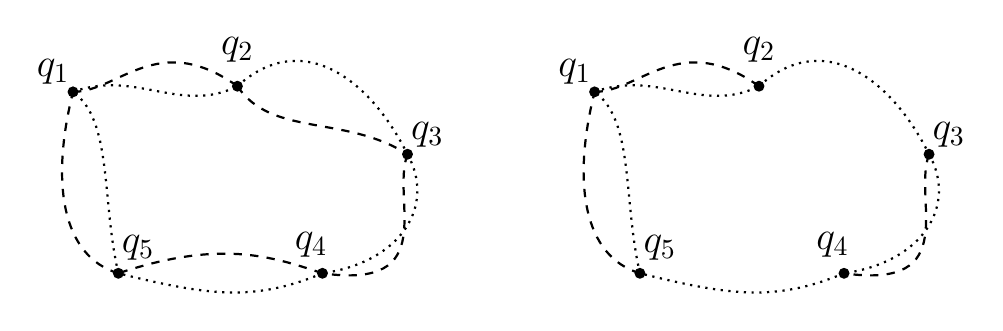
\begin{tikzpicture}[
    scale=0.72,
    vertex/.style={circle, fill=black, inner sep=1.4pt},
    lab/.style={font=\Large}
]

% ==================================================

% First copy

% ==================================================

\coordinate (a1) at (-3.2,  1.1);
\coordinate (a2) at (-0.3,  1.2);
\coordinate (a3) at ( 2.7,  0.0);
\coordinate (a4) at ( 1.2, -2.1);
\coordinate (a5) at (-2.4, -2.1);

% q1 to q2
\draw[dashed, thick]
  (a1) .. controls (-2.4,1.1) and (-1.7,2.2) .. (a2);

\draw[dotted, thick]
  (a1) .. controls (-2.1,1.5) and (-1.3,0.7) .. (a2);

% q2 to q3
\draw[dashed, thick]
  (a2) .. controls (0.3,0.3) and (1.6,0.7) .. (a3);

\draw[dotted, thick]
  (a2) .. controls (0.8,2.2) and (2.0,1.4) .. (a3);

% q3 to q4
\draw[dashed, thick]
  (a3) .. controls (2.4,-0.8) and (3.3,-2.4) .. (a4);

\draw[dotted, thick]
  (a3) .. controls (3.2,-0.9) and (2.6,-1.9) .. (a4);

% q4 to q5
\draw[dashed, thick]
  (a4) .. controls (0.3,-1.8) and (-0.6,-1.5) .. (a5);

\draw[dotted, thick]
  (a4) .. controls (0.0,-2.6) and (-0.8,-2.5) .. (a5);

% q5 to q1
\draw[dashed, thick]
  (a5) .. controls (-3.4,-1.8) and (-3.6,-0.5) .. (a1);

\draw[dotted, thick]
  (a5) .. controls (-2.7,-0.8) and (-2.5,0.6) .. (a1);

% vertices
\node[vertex] at (a1) {};
\node[vertex] at (a2) {};
\node[vertex] at (a3) {};
\node[vertex] at (a4) {};
\node[vertex] at (a5) {};

% labels
\node[lab] at (-3.55,  1.45) {$q_1$};
\node[lab] at (-0.30,  1.85) {$q_2$};
\node[lab] at ( 3.05,  0.35) {$q_3$};
\node[lab] at ( 1.00, -1.60) {$q_4$};
\node[lab] at (-2.05, -1.65) {$q_5$};

% ==================================================

% Second copy

% Shifted 7.2 units to the right

% ==================================================

\begin{scope}[xshift=2cm]
\coordinate (b1) at (4.0,  1.1);
\coordinate (b2) at (6.9,  1.2);
\coordinate (b3) at (9.9,  0.0);
\coordinate (b4) at (8.4, -2.1);
\coordinate (b5) at (4.8, -2.1);

% q1 to q2
\draw[dashed, thick]
  (b1) .. controls (4.8,1.1) and (5.5,2.2) .. (b2);

\draw[dotted, thick]
  (b1) .. controls (5.1,1.5) and (5.9,0.7) .. (b2);

% q2 to q3
\draw[dotted, thick]
  (b2) .. controls (8.0,2.2) and (9.2,1.4) .. (b3);

% q3 to q4
\draw[dashed, thick]
  (b3) .. controls (9.6,-0.8) and (10.5,-2.4) .. (b4);

\draw[dotted, thick]
  (b3) .. controls (10.4,-0.9) and (9.8,-1.9) .. (b4);

% q4 to q5
\draw[dotted, thick]
  (b4) .. controls (7.2,-2.6) and (6.4,-2.5) .. (b5);

% q5 to q1
\draw[dashed, thick]
  (b5) .. controls (3.8,-1.8) and (3.6,-0.5) .. (b1);

\draw[dotted, thick]
  (b5) .. controls (4.5,-0.8) and (4.7,0.6) .. (b1);

% vertices
\node[vertex] at (b1) {};
\node[vertex] at (b2) {};
\node[vertex] at (b3) {};
\node[vertex] at (b4) {};
\node[vertex] at (b5) {};

% labels
\node[lab] at (3.65,  1.45) {$q_1$};
\node[lab] at (6.90,  1.85) {$q_2$};
\node[lab] at (10.25, 0.35) {$q_3$};
\node[lab] at (8.20, -1.60) {$q_4$};
\node[lab] at (5.15, -1.65) {$q_5$};
\end{scope}

\end{tikzpicture}
\caption{The left figure shows a $5$-arithmetic rope, while the right figure shows a quasi-$5$-arithmetic rope. Dotted lines represent odd-length paths, and dashed lines represent even-length paths. Note that the pairwise $G$-distance between the $q_i$'s is at least $5$ for arithmetic ropes and at least $6$ for quasi-arithmetic ropes.}
\label{fig:arithmetic_comparison}
\end{figure}

\section{Constructing a quasi-arithmetic rope}
\label{sec:quasi_arithmetic_rope}

In the remainder of this paper, we will make repeated use of the fact that $N^{k}[v]$ is bipartite for every vertex $v$ whenever $G$ has odd girth at least $2k + 3$ (see~\cite[Obs. 2.3]{chudnovsky2024colouringtperfectgraphs}).
In what follows, we say that a vertex set $B$ covers $C$ if $ B$ and $ C$ are disjoint and every vertex in $C$ has a neighbor in $B$. Moreover, we say that a vertex set $X$ is anticomplete to a vertex set $Y$ if every vertex in $X$ has no neighbor in $Y$.

In analogy to~\cite{chudnovsky2024colouringtperfectgraphs}, let us consider the notion of a \emph{broken quasi-$r$-arithmetic rope}, which consists of vertices $q_1, \dots, q_{r + 1}$ together with paths $Q_{i, 1}, Q_{i, 2}$ for $i \in [r]$ such that 

\begin{itemize}
    \item each $Q_{i, 1}$ and $Q_{i, 2}$ is a $q_iq_{i+1}$-path,
    \item each $Q_{i, 1}$ has odd length,
    \item for every $h \in \{1, 2\}^r$, $Q_{1, h_1} \cup \dots \cup Q_{r, h_r}$ is an induced path, and
    \item the vertices $q_1, \dots, q_{r + 1}$ are pairwise at $G$-distance at least 6.
\end{itemize}

We call a broken quasi-$r$-arithmetic rope \emph{alternating} if $Q_{i, 2}$ has even length whenever $i \in [r]$ is even, and call it \emph{good} if, in addition, $Q_{r,2}$ has even length.
Clearly, the two notions are equal if $r$ is even.
We will prove the following.

\begin{lemma}\label{lemma:construction_almost_broken}
    Let $r \geq 1$, let $G$ be a graph with odd girth at least 15, and let $B, C \subseteq V(G)$ be disjoint with $B$ covering $C$. Let $q_1 \in V(G) \setminus C$ be a vertex such that $G[C \cup \{q_1\}]$ is connected and $\chi(C) \geq 11 \left\lfloor \frac{r}{2} \right\rfloor + 5 \left\lceil \frac{r}{2} \right\rceil + c$. Then there exists $B' \subseteq B, C' \subseteq C, q_2, q_3, \dots, q_{r + 1} \in C \setminus C'$ and an alternating broken quasi-$r$-arithmetic rope $R$ on vertices $q_1,\dots,q_{r+1}$ with paths $(Q_{i, 1}, Q_{i, 2})_{i = 1}^r$ such that 
    \begin{itemize}
        \item $G[C' \cup \{q_{r + 1}\}]$ is connected,
        \item $\chi(C') \geq c$,
        \item $B'$ covers $C'$,
        \item $B'$ is anticomplete to $(V(Q_{i, 1}) \cup V(Q_{i, 2})) \setminus N^3[q_{i + 1}]$ for   all $i \in [r]$,
        \item $(V(Q_{i, 1}) \cup V(Q_{i, 2})) \setminus N^2[q_{i + 1}] \subseteq C \cup \{q_1\}$ for all $i \in [r]$,
        \item $C'$ is anticomplete to $\left( \bigcup_{i = 1}^r (V(Q_{i, 1}) \cup V(Q_{i, 2})) \right) \setminus \{q_{r + 1}\}$, and
        \item the $G$-distance between $\{q_1, \dots, q_{r}\}$ and $C' \cup \{q_{r+  1}\}$ is at least $6$. 
    \end{itemize}
    If $\chi(C) \geq 11 \left\lceil \frac{r}{2} \right\rceil + 5 \left\lfloor \frac{r}{2} \right\rfloor + c$, then $R$ can even be chosen to be good.
\end{lemma}

Let us first explain how the above statement yields our main claim.

\begin{proof}[Proof of \Cref{thm:quasi_rope_existence}]
    Let $G$ be a graph with odd girth at least 15 and let $X \subseteq V(G)$ with 
    \[\chi(X) \geq \begin{cases}
        16r + 5 & \text{if } r \text{ is even,}\\
        16r + 11 & \text{if } r \text{ is odd.}
    \end{cases}\]
Without loss of generality, we may assume that $X$ is connected as otherwise we can choose a connected component of $X$ with maximum chromatic number. 
Let $v$ be some vertex of $X$ and let $L_i = N^i_X(v)$ for all $i \geq 0$. Since $G$ has odd girth at least 15, there is an integer $s \geq 6$ such that $\chi(L_{s + 1}) \geq \lceil \chi(X) /2 \rceil$.
Hence if $r$ is even, we have
\[
\chi(L_{s + 1}) \geq \left\lceil \frac{\chi(X)}{2} \right \rceil \geq 8r + 3 = 11 \left \lceil \frac{r}{2} \right \rceil + 5 \left \lfloor \frac{r}{2} \right \rfloor + 3,
\]
and if $r$ is odd, we have
\[
\chi(L_{s + 1}) \geq \left\lceil \frac{\chi(X)}{2} \right \rceil \geq 8r + 6 = 11 \left \lceil \frac{r}{2} \right \rceil + 5 \left \lfloor \frac{r}{2} \right \rfloor + 3.
\]

Let $C$ be the set of vertices of a connected component of $G[L_{s + 1}]$ with maximum chromatic number. Let $q_1$ denote a vertex of $L_s$ that is adjacent to some vertex of $C$ and let $B = L_s$. \Cref{lemma:construction_almost_broken} implies that there exists $B' \subseteq B, C' \subseteq C$, and a good broken quasi-$r$-arithmetic rope consisting of ends $q_1$ and $q_2, \dots, q_{r + 1} \in C \setminus C'$ and paths $Q_{i, 1}$ and $Q_{i, 2}$ for each $i \in [r]$ such that 
\begin{itemize}
    \item $G[C' \cup \{q_{r+ 1} \}]$ is connected,
    \item $\chi(C') \geq 3$,
    \item $B'$ covers $C'$,
    \item $B'$ is anticomplete to $(V(Q_{i, 1}) \cup V(Q_{i, 2})) \setminus N^3[q_{i + 1}]$ for   all $i \in [r]$,
    \item $V(Q_{i, 1}) \cup V(Q_{i, 2})$ is contained in $C \cup \{q_1\} \cup (B \cap N^2[q_{i + 1}])$ for all $i \in [r]$,
    \item $C'$ is anticomplete to $\left( \bigcup_{i = 1}^r (V(Q_{i, 1}) \cup V(Q_{i, 2})) \right) \setminus \{q_{r + 1}\}$, and
    \item the $G$-distance between $\{q_1, \dots, q_{r}\}$ and $C' \cup \{q_{ r+  1}\}$ is at least $6$. 
\end{itemize}
Since $\chi(C') \geq 3$ and $\chi(N^5_G[q_{r + 1}]) \leq 2$, there exists a vertex $x \in C'$ with $G$-distance at least $6$ from $q_{r + 1}$. Since $x \in C'$, it also has $G$-distance at least $6$ from $q_1, \dots, q_r$. As $B'$ covers $C'$, there is a vertex $b \in B'$ adjacent to $x$. 

Let $P_1$ be a shortest path between $q_{r + 1}$ and $b$ in $G[\{q_{r + 1}, b \} \cup C']$. Observe that this is an induced path.
Now let $a_1 \in L_{s-1}$ be a vertex adjacent to $q_1$ and let $a_2 \in L_{s - 1}$ be a vertex adjacent to $b$.
Let $P_2$ be an induced path between $a_1$ and $a_2$ in $G\left[ \{a_1, a_2\} \cup \bigcup_{i = 0}^{s - 2} L_i \right]$. We claim that $ba_2P_2a_1q_1$ is again an induced path. It suffices to show that $\{b , a_2\}$ is anticomplete to $\{a_1, q_1\}$ since $V(P_2) \setminus \{a_1, a_2\} \subseteq \bigcup_{i = 0}^{s - 2} L_i$. This follows because the $G$-distance between vertices in $\{b, a_2\}$ and $x$ is at most $2$, but the $G$-distance between vertices in $\{a_1, q_1\}$ and $x$ is at least $5$.

Now let $P$ be the induced path $P_1ba_2P_2a_1q_1$ between $q_{r + 1}$ and $q_1$. To prove that $P$ is in fact an induced path, we only need to show that $V(P_1) \setminus \{b\}$ is anticomplete to $\{q_1\}$ since $V(P_1) \setminus \{b\} \subseteq C \subseteq L_{s + 1}$ and $V(P_2) \subseteq L_{s - 1}$. This holds true because $V(P_1) \setminus \{b\} \subseteq C' \cup \{q_{r + 1}\}$ and the $G$-distance between $q_1$ and $C' \cup \{q_{r + 1}\}$ is at least 6.

Finally, we show that $V(P) \setminus \{q_1, q_{r + 1}\}$ is anticomplete to $\bigcup_{i = 1}^r (V(Q_{i, 1}) \cup V(Q_{i, 2})) \setminus \{q_1, q_{r + 1}\}$. For $V(P_1) \setminus \{q_{r + 1}, b\} \subseteq C'$, the claim follows directly from \Cref{lemma:construction_almost_broken}. Since $V(P_2) \setminus \{a_1, a_2\} \subseteq \bigcup_{i = 0}^{s - 2} L_i$ and $V(P_1) \subseteq L_s \cup L_{s + 1}$, we only need to show that $\{a_1, a_2, b\}$ is anticomplete to $\bigcup_{i = 1}^r (V(Q_{i, 1}) \cup V(Q_{i, 2})) \setminus \{q_1, q_{r + 1}\}$. 

Since $a_1, a_2 \in L_{s - 1}$ and $(V(Q_{i, 1}) \cup V(Q_{i, 2})) \setminus\{q_1\} \subseteq C \cup (B \cap N^2[q_{i + 1}])$ for all $i \in [r]$, $a_1$ and $a_2$ may only have a neighbor in $B \cap N^2[q_{i + 1}]$ along $Q_{i, 1} \cup Q_{i, 2}$. Since $a_1$ and $a_2$ each have $G$-distance at least $4$ to $\{q_2, \dots, q_{r + 1}\}$, the respective anti-completeness condition follows.
Since $b \in B'$ and $B'$ is anticomplete to $(V(Q_{i, 1}) \cup V(Q_{i, 2})) \setminus N^3[q_{i + 1}]$ for all $i \in [r]$, the respective anti-completeness condition follows because $b$ has $G$-distance at least $5$ to $\{q_1, \dots, q_{r + 1}\}$.

Hence we obtain a quasi-$r$-arithmetic rope from the good broken quasi-$r$-arithmetic rope by extending $Q_{r, 1}$ and $Q_{r,2}$ with $P$. Note that we might need to relabel $Q_{r, 1}$ and $Q_{r, 2}$ depending on the parity of $P$, which is possible because the broken quasi-$r$-arithmetic rope is good.
\end{proof}

The broken quasi-arithmetic ropes in \Cref{lemma:construction_almost_broken} are constructed inductively.
Each step is based on the following result, which can be seen as a refinement of \cite[Lem. 4.4]{chudnovsky2024colouringtperfectgraphs}.

\begin{lemma}\label{lemma:contruction_two_paths_optimal}
    Let $c \geq 1$ and let $G$ be a graph with odd girth at least $13$, let $B, C \subseteq V(G)$ be disjoint vertex subsets with $B$ covering $C$, let $q \in V(G) \setminus C$ be a vertex such that $G[C \cup \{q\}]$ is connected and $\chi(C)\geq c+11$.

    Then there exists $B' \subseteq B, C' \subseteq C, q' \in C \setminus C'$ and two induced paths $Q_1, Q_2$ between $q$ and $q'$ in $G[(C \setminus C') \cup (B \setminus B') \cup \{q\}]$ such that 

    \begin{itemize}
        \item $G[C' \cup \{q'\}]$ is connected,
        \item $\chi(C') \geq c$, 
        \item $B'$ covers $C'$,
        \item $B'$ is anticomplete to $(V(Q_1) \cup V(Q_2)) \setminus N^3[q']$,
        \item $V(Q_1) \cup V(Q_2)$ is contained in $C \cup \{q\} \cup ((B \cap N^2[q']) \setminus N^4[q])$,
        \item $C'$ is anticomplete to $(V(Q_1) \cup V(Q_2)) \setminus \{q'\}$,
        \item the $G$-distance between $q$ and $C' \cup \{q'\}$ is at least $6$, and
        \item $Q_1$ has odd length and $Q_2$ has even length.
    \end{itemize}
\end{lemma}

For segments of the broken quasi-arithmetic rope that don't require an even-length path, we make use of the following variant that requires a weaker bound on the chromatic number at the cost of a slightly higher odd girth.

\begin{lemma}\label{lemma:construction_quasi}
    Let $c \geq 1$ and let $G$ be a graph with odd girth at least $15$, let $B, C \subseteq V(G)$ be disjoint vertex subsets with $B$ covering $C$, let $q \in V(G) \setminus C$ be a vertex such that $G[C \cup \{q\}]$ is connected and $\chi(C)\geq c+5$.

    Then there exists $B' \subseteq B, C' \subseteq C, q' \in C \setminus C'$ and an induced odd-length path $Q_1$ between $q$ and $q'$ in $G[(C \setminus C') \cup (B \setminus B') \cup \{q\}]$ such that 

    \begin{itemize}
        \item $G[C' \cup \{q'\}]$ is connected,
        \item $\chi(C') \geq c$, 
        \item $B'$ covers $C'$,
        \item $B'$ is anticomplete to $V(Q_1) \setminus N^3[q']$,
        \item $V(Q_1)$ is contained in $C \cup \{q\} \cup ((B \cap N^2[q']) \setminus N^4[q])$,
        \item $C'$ is anticomplete to $V(Q_1) \setminus \{q'\}$, and
        \item the $G$-distance between $q$ and $C' \cup \{q'\}$ is at least $6$.
    \end{itemize}
\end{lemma}

We close this section by showing how \Cref{lemma:construction_almost_broken} is obtained from the above two lemmas.
Their proofs will be discussed in the next two sections.

\begin{proof}[Proof of \Cref{lemma:construction_almost_broken}]

    We prove the first claim by induction and explain how it implies the second.
    The base case $r = 1$ follows from \Cref{lemma:construction_quasi}. Now let $r \geq 2$ and assume that the claim holds up to $r - 1$, i.e., there exists $B_{r-1} \subseteq B, C_{r - 1} \subseteq C, q_2, q_3, \dots, q_r \in C \setminus C_{r- 1}$, and an alternating broken quasi-$(r-1)$-arithmetic rope $(q_i, Q_{i, 1}, Q_{i, 2})_{i = 1}^{r - 1}$ satisfying the above properties with $c' =  5 + c$ if $r$ is odd or with $c' = 11 + c$ if $r$ is even.
    
    Depending on the parity of $r$, \Cref{lemma:contruction_two_paths_optimal} or \Cref{lemma:construction_quasi} with $B_{r-1}, C_{r-1}$, and $q_r$ implies that there are $B' \coloneqq B_r, C' \coloneqq C_r \subseteq C_{r - 1}, q_{r + 1} \in C_{r - 1} \setminus C_r$, and two induced paths $Q_{r, 1}, Q_{r,2}$ between $q_r$ and $q_{r + 1}$ in $G\left[ (C_{r - 1} \setminus C_r ) \cup (B_{r - 1} \setminus B_r) \cup \{q_{r}\} \right]$ satisfying the properties of the respective lemma. (Note that $Q_{r, 2}$ does not have to be an even-length path if $r$ is odd). 
    It is easy to check that the properties listed above are satisfied. We only need to verify that $(q_i, Q_{i, 1}, Q_{i, 2})_{i = 1}^r$ is in fact an alternating broken quasi-$r$-arithmetic rope. It remains to check that the induced path condition holds since the rest is immediate.
    
    To this end, suppose for contradiction that there is some $(h_1, \dots, h_r)$ such that $Q_{1, h_1} \cup Q_{2, h_2 } \cup \dots \cup Q_{r, h_r}$ is not an induced path.
    By the induction hypothesis, $Q_{1, h_1} \cup Q_{2, h_2 } \cup\dots \cup Q_{r - 1, h_{r - 1}}$ is an induced path. Hence there is an edge between two vertices $x \in V(Q_{i, h_{i}})$ and $y \in V(Q_{r, h_r}) \setminus \{q_r\}$ for some $i \in [r - 1]$. Since $C_{r - 1}$ is anticomplete to $(V(Q_{i, 1}) \cup V(Q_{i, 2})) \setminus \{q_r\}$, we have that $y \in (B_{r - 1} \cap N^2[q_{r + 1}]) \setminus N^4[q_r]$. Since $B_{r - 1}$ is anticomplete to $(V(Q_{i, 1}) \cup V(Q_{i, 2})) \setminus N^3[q_{i + 1}]$, we have that $x \in N^3[q_{i + 1}]$. Hence there is a path of length at most 4 between $y$ and $q_{i + 1}$, which implies that $y \neq q_{r + 1}$. 
    
    Now suppose that $y$ does not have a neighbor in $C_{r - 1} \cap V(Q_{r,    h_r})$. Note that this implies that $y \in N^2(q_{r+1})$ since $q_{r + 1} \in C_{r - 1}$. Since $V(Q_{r, h_r}) \subseteq C_{r - 1} \cup \{q_r\} \cup (B \cap N^2[q_{r + 1}])$, $y$ has two neighbors in $V(Q_{r, h_r}) \cap (B \cap N^2[q_{r + 1}])$, which we denote as $z_1$ and $z_2$. At most one of these can be adjacent to $q_{r +1 }$ since $V(Q_{r, h_r})$ is an induced path. Without loss of generality, we may say that $z_1 \in N^2(q_{r + 1})$. Since $G$ is triangle-free, there is a vertex $b_{y}$ adjacent to $y$ and $q_{r + 1}$ and a vertex $b_{z_1}$ adjacent to $z_1$ and $q_{r + 1}$. However, together with $q_{r + 1}$ these vertices form a cycle of length 5, which contradicts that the odd girth of $G$ is at least $7$. Thus $y$ has a neighbor in $C_{r - 1} \cap V(Q_{r, h_r})$.
    
    Therefore if $i < r - 1$, there is a path of length at most 5 from $q_{i + 1}$ to a vertex in $C_{r - 1}$, which contradicts the induction hypothesis that the $G$-distance between $q_{i + 1}$ and $C_{r - 1}$ is at least 6. If $i = r - 1$, the $G$-distance between $q_r$ and $y$ is at most 4, which is again a contradiction.

    The second claim for good broken quasi-$r$-arithmetic ropes is equivalent to the first if $r$ is even. For odd $r$, the second claim follows from the first for $r-1$ and \Cref{lemma:contruction_two_paths_optimal} by arguing exactly as above. 
\end{proof}

\section{Constructing segments with odd and even paths}
\label{sec:segments_odd_and_even}

\begin{definition}
    A stable grading is a sequence $(W_1, \dots, W_n)$ of pairwise disjoint stable sets of $V(G)$ such that their union is $V(G)$.
    
    A vertex $u \in V(G)$ is earlier than $v \in V(G)$ with respect to a stable grading $(W_1, \dots, W_n)$ if $u \in W_i$ and $v \in W_j$ for some $i < j$.
\end{definition}

We say that a vertex $w \in V(G)$ is left-active with respect to a vertex set $X$ if there exists an edge $uv$ of $G[X]$ such that $u$ and $v$ are earlier than $w$ and $w$ is adjacent to at least one of $u$ and $v$.

\begin{lemma}\label{lemma1:beyond_leveling}
    Let $c \geq 1$ and let $G$ be a graph with $\chi(G) \geq c + 8$ and $V(G) = C_0 \cup C_1 \cup C_2$.
    Furthermore, let \((C_0^t)_{t\geq 1}\) be a partition of \(C_0\) such that the ends of every edge of \(G[C_0]\) lie in parts whose indices differ by at most one.

    If $(W_1, \dots, W_n)$ is a stable grading of $V(G)$, there exists a subset $X$ of $V(G)$ and an edge $uv$ belonging to one of $G[C_1], G[C_2]$, or $G[C_0^t]$, for some $t \geq 1$, such that
    \begin{itemize}
        \item $G[X]$ is connected,
        \item $\chi(X) \geq c$,
        \item $u$ and $v$ are earlier than every vertex in $X$, and
        \item at least one of $u$ and $v$ has a neighbor in $X$.
    \end{itemize}
        \end{lemma}


\begin{proof}
    Let $A$ be the set of vertices in $G$ that are left-active with respect to $C_1, C_2,$ or $C_0^t$ for some $t \geq 1$. 

    \textbf{Case 1:} $\chi(A) \geq c$.
    Let $D$ be a connected component of $G[A]$ with maximum chromatic number. Note that we have $\chi(D) = \chi(A) \geq c$. Then there is a minimal integer $i$ such that $1 \leq i \leq n$ and $W_i \cap V(D)$ is non-empty. Let $w$ be a vertex in $W_i \cap V(D)$. Since $w$ is left-active, there is an edge $uv$ of $G[C_1], G[C_2]$ or $G[C_0^t]$, for some $t \geq 1$, such that $u$ and $v$ are earlier than $w$ and $w$ is adjacent to one of $u$ and $v$. Since $i$ was chosen to be minimal, $u$ and $v$ are earlier than every vertex in $D$. Thus $X = V(D)$ satisfies the required conditions.

    \textbf{Case 2:} $\chi(A) \leq c - 1$.
    Let $B_h = C_h \setminus A$ for $h \in \{0, 1, 2\}$. We perform a case distinction depending on which $B_h$ has a sufficiently large chromatic number.
    Since 
    \[\chi(B_0 \cup B_1 \cup B_2) \geq \chi(G) - \chi(A) \geq c + 8 - (c -1) = 9,\]
    we either have $\chi(B_0) \geq 5$ or $\chi(B_1 \cup B_2) \geq 5$. In the second case, one of $B_1$ or $B_2$ must have chromatic number at least $3$.

    \textbf{Case 2.1:} $\chi(B_0) \geq 5$.
    Since distinct same-parity parts among the \(C_0^t\)'s are anticomplete in \(G[C_0]\), there is an integer $r \geq 1$ with $\chi(B_0 \cap C_0^{r}) \geq \left\lceil \chi(B_0) / 2 \right\rceil \geq 3$.
    Hence \(G[B_0 \cap C_0^r]\) contains an odd cycle \(D\) as a subgraph. Since each \(W_i\) is stable, the endpoints of every edge of \(D\) lie in different parts of the stable grading. Orient each edge from the earlier endpoint to the later endpoint, and denote the resulting orientation by \(\vec D\).

    Since no vertex in \(D\) is left-active with respect to \(C_0^r\), there is no directed path of length \(2\) in \(\vec D\). Indeed, if \(u \to v \to w\) is such a path, then \(uv\) is an edge of \(G[C_0^r]\), both \(u\) and \(v\) are earlier than \(w\), and \(w\) is adjacent to \(v\), contradicting \(w\in B_0\).
    Hence every vertex of \(\vec D\) is either a sink or a source. Thus the sources and sinks form a bipartition of \(D\), contradicting that \(D\) is an odd cycle. 

    \textbf{Case 2.2:} $\chi(B_h) \geq 3$ for some $h \in \{1, 2\}$.
    The same orientation argument applied to an odd cycle in \(G[B_h]\) gives a contradiction, since no vertex of \(B_h\) is left-active with respect to \(C_h\).
\end{proof}

In the triangle-free case, we can prove the following lemma. Its proof is identical to the proof of~\cite[Lemma 4.3]{chudnovsky2024colouringtperfectgraphs}. We include it for the sake of completeness.

\begin{lemma}\label{lemma2:beyond_leveling}
    Let $c \geq 1$ and let $G$ be a triangle-free graph with $\chi(G) \geq c + 9$ and $V(G) = C_0 \cup C_1 \cup C_2$. Furthermore, let \((C_0^t)_{t\geq 1}\) be a partition of \(C_0\) such that the ends of every edge of \(G[C_0]\) lie in parts whose indices differ by at most one.

    If $(W_1, \dots W_n)$ is a stable grading of $V(G)$, there exists a subset $X$ of $V(G)$ and an edge $uv$ belonging to one of $G[C_1], G[C_2]$, or $G[C_0^t]$, for some $t \geq 1$, such that
    \begin{itemize}
        \item $G[X]$ is connected,
        \item $\chi(X) \geq c$,
        \item $u$ and $v$ are earlier than every vertex in $X$, 
        \item $u$ has no neighbor in $X$, and
        \item $v$ has a neighbor in $X$.
    \end{itemize}
    \end{lemma}

\begin{proof}
By \Cref{lemma1:beyond_leveling}, there exists a subset $X'$ of $V(G)$ and an edge $u'v'$ of $G[C_1], G[C_2]$, or $G[C_0^t]$ for some $t \geq 1$ with the following properties:  
\begin{itemize}
    \item $G[X']$ is connected,
    \item $\chi(X') \geq c + 1$,
    \item $u'$ and $v'$ are earlier than every vertex in $X'$, 
    \item $v'$ has a neighbor in $X'$.
\end{itemize}

Let $D$ be a connected component of $G[X' \setminus N(v')]$ with maximum chromatic number. Since $G$ is triangle-free, we have that 
\[\chi(D) \geq \chi(X') - \chi(N(v')) \geq \chi(X') - 1 \geq c.\]
If $u'$ has a neighbor in $V(D)$, then the lemma follows by setting $u = v', v = u'$, and $X = V(D)$. Hence, we may assume that $u'$ has no neighbor in $V(D)$. Let $w$ be a neighbor of $v'$ in $X'$ that has a neighbor in $V(D)$. Note that $w$ is non-adjacent to $u'$ since $G$ is triangle-free. The lemma follows by setting $u = u', v = v'$, and $X = V(D) \cup \{w\}$.
\end{proof}

We are now ready to prove \Cref{lemma:contruction_two_paths_optimal}.

\begin{proof}[Proof of \Cref{lemma:contruction_two_paths_optimal}]
For $i \geq 0$, let $M_i$ denote the set of vertices in $C \cup \{q\}$ with $G[C \cup \{q\}]$-distance exactly $i$ from $q$. Since $G$ has odd girth at least $13$, we have that $\chi(M_0 \cup \dots \cup M_5) \leq \chi(N_G^5[q]) \leq 2$. Let $d$ be the unique integer such that $M_{d} \neq \emptyset$ and $M_{d'} = \emptyset$ for all $d' > d$.

\textbf{Finding structure in $B$ and $C$: }

For $1 \leq t \leq d$, let $\mathcal{M}^{\leq t}  = M_0 \cup M_1 \cup \dots \cup M_t$ and $\mathcal{M}^{\geq t} = M_{t} \cup M_{t + 1} \cup \dots \cup M_{d}$.
For \(6 \leq t \leq d\), partition \(B\) into three sets \(B_0^t, B_1^t, B_2^t\) as follows. Let \(B_0^t\) be the set of vertices in \(B\) with no neighbor in \(\mathcal M^{\le t-3}\). Let \(B_1^t\) be the set of vertices \(v \in B\) with a neighbor in \(\mathcal M^{\le t-3}\) for which the \(G[\mathcal M^{\le t-3} \cup \{v\}]\)-distance between \(q\) and \(v\) is odd, and let \(B_2^t\) be the set of vertices for which this distance is even.

For each $6 \le t \le d$, let $C_0^t$ be the set of vertices in
$M_t \setminus N_G^5[q]$ that have a neighbor in $B_0^t$ but no neighbor
in $B_1^t \cup B_2^t$. For $i=1,2$, let $C_i^t$ be the set of vertices
in $M_t \setminus N_G^5[q]$ that have a neighbor in $B_i^t$. Finally, set $C_i = \bigcup_{t=6}^{d} C_i^t$ for each $i \in \{0, 1, 2\}$.
Since $B$ covers $C$, it follows that $C \setminus N_G^5[q] = C_0 \cup C_1 \cup C_2$, and that $B_i^t$ covers $C_i^t$ for every $6 \le t \le d$ and $i \in \{0, 1, 2\}$.
Note that we have that $B_0^t \supseteq B_0^{t + 1}$ and $B_h^t \subseteq B_h^{t + 1}$ for all $h \in \{1, 2\}$ and $6 \leq t \leq d - 1$.

\textbf{Constructing a suitable stable grading: }

The constructed stable grading is illustrated in \Cref{fig:grading}.

\begin{figure}[ht]
    \centering
    \includegraphics[width=0.9\linewidth]{grading_new.png}
    \caption{An illustration of the stable grading of $C$ constructed in the proof of \Cref{lemma:contruction_two_paths_optimal}. Think of it as follows: inside a level $M_i$, a vertex is earlier than another if it is in a "lower" part of the stable grading. Any $W_j$ intersecting $\mathcal{M}^{\leq t}$ for some $t$ is earlier than any $W_{j'}$ that does not intersect $\mathcal{M}^{\leq t}$.}
    \label{fig:grading}
\end{figure}
Let \(n_t = \lvert M_t \rvert\) and set \(s_t = \sum_{i = 0}^{t} n_i\). Let \(m_1, \dots, m_{s_{d - 1}}\) be an ordering of the vertices in \(\mathcal{M}^{\leq d - 1}\) such that, whenever \(1 \leq i < j \leq s_{d - 1}\), the \(G[\mathcal{M}^{\leq d -1}]\)-distance between \(q\) and \(m_i\) is at most the \(G[\mathcal{M}^{\leq d - 1}]\)-distance between \(q\) and \(m_j\).

We first construct a stable grading of $C_1 \cup C_2$. We begin with the case \( t = 6 \).
For \(1 \leq i \leq s_{3}\), let \(W_i^{(6)}\) be the set of vertices \(v\) in \(\mathcal{M}^{\geq 6}\) such that \(v\) has a neighbor in \(B_1^6 \cup B_2^6\) that is adjacent to \(m_i\), and has no neighbor in \(B_1^6 \cup B_2^6\) adjacent to any of \(m_1, \dots, m_{i - 1}\).

For \(7 \leq t \leq d\) and \(1 \leq i \leq n_{t - 3}\), let \(W_i^{(t)}\) be the set of vertices \(v\) in \(\mathcal{M}^{\geq t}\) such that \(v\) has a neighbor in \(B_1^t \cup B_2^t\) that is adjacent to \(m_{i + s_{t - 4}} \in M_{t - 3}\) and no neighbor in \(B_1^t \cup B_2^t\) that is adjacent to one of \(m_1, \dots, m_{(i -1 ) + s_{t - 4}}\).

Each set $W_i^{(t)}$ is stable since \(G\) has odd girth at least \(7\). 
Hence, ordered lexicographically by \(t\) and then by \(i\), the sets
\[
\left(W_1^{(6)}, \dots, W_{s_{3}}^{(6)}, W_1^{(7)}, \dots, W_{n_4}^{(7)}, \dots, W^{(d)}_1, \dots, W^{(d)}_{n_{d - 3}}\right)
\]
form a stable grading of \(C_1 \cup C_2\).

We now construct a stable grading of \(C_0\).
For \(6 \leq t \leq d\) and \(1 \leq i \leq n_{t - 1}\),
let \(\widetilde{W}^{(t)}_i\) be the set of vertices in \(C_0^t\) that are adjacent to \(m_{i + s_{t - 2}}\), and are non-adjacent to \(m_1, \dots, m_{(i - 1) + s_{t - 2}}\). 
Since \(G\) is triangle-free, the sets
\[
\left(\widetilde{W}^{(6)}_1, \dots, \widetilde{W}_{n_5}^{(6)}, \dots, \widetilde{W}_{1}^{(d)}, \dots, \widetilde{W}_{n_{d - 1}}^{(d)}\right)
\]
form a stable grading of \( C_0 \).

By combining these stable gradings, we get that
\[
\left(W_A, W_B, W^{(6)}_1, \dots, W_{s_{3}}^{(6)}, \widetilde{W}^{(6)}_1, \dots, \widetilde{W}^{(6)}_{n_5}, \dots,  W_1^{(d)}, \dots, W_{n_{d - 3}}^{(d)}, \widetilde{W}_1^{(d)}, \dots, \widetilde{W}_{n_{d - 1}}^{(d)} \right)
\]
is a stable grading of $C$, where $(W_A, W_B)$ is any bipartition of $C \cap N_G^5[q]$. When convenient, we regard the same sequence, with \( W_A\) and \( W_B\) omitted, as a stable grading of \( C \setminus N^5_G[q]\).

\textbf{Constructing an odd- and even-length path:}

From \Cref{lemma2:beyond_leveling} and $\chi(C \setminus N_G^5[q]) \geq \chi(C) - 2 \geq c + 9$, we get that there exists a subset $C'$ of $C \setminus N_G^5[q]$ and an edge $u'q'$ of $G[C_1], G[C_2]$ or $G[C_0^t]$, for some $t \geq 6$, with the following properties:

\begin{itemize}
    \item $G[C' \cup \{q'\}]$ is connected,
    \item $\chi(C') \geq c$,
    \item $u'$ and $q'$ are earlier than every vertex in $C'$, and
    \item $u'$ has no neighbor in $C'$.
\end{itemize}

Observe that the $G$-distance between $q$ and any vertex in $C' \cup \{u', q'\}$ is at least \(6\).
We perform a case distinction according to which of the above induced subgraphs contains the edge \(u'q'\).

\textbf{Case 1:} $u'q'$ is an edge of $G[C_0^t]$ for some $6 \leq t \leq d$.
The situation is illustrated in~\Cref{fig:case1_arithmetic}.
\begin{figure}
    \centering
    \includegraphics[width=0.9\linewidth]{case1_arithmetic_new.png}
    \caption{A possible situation in case 1 of the proof of \Cref{lemma:contruction_two_paths_optimal}.}
    \label{fig:case1_arithmetic}
\end{figure}
Let $i_{u'}$  and \(i_{q'}\) be such that $u' \in \widetilde{W}^{(t)}_{i_{u'}}$ and $q' \in \widetilde{W}^{(t)}_{i_{q'}}$.
Let $Q_{u'}$ be an induced path in $G[\mathcal{M}^{\leq t - 2} \cup \{m_{i_{u'} + s_{t - 2}}, u'\}]$ between $q$ and $u'$ of length $t$ and let $Q_{q'}$ be an induced path in $G[\mathcal{M}^{\leq t -2} \cup \{m_{i_{q'} + s_{t - 2}}, q'\}]$ between $q$ and $q'$ of length $t$. 
Let \(Q_{u'q'}\) be the path of length \(t + 1\) between $q$ and $q'$ obtained by extending $Q_{u'}$ by the edge $u'q'$. This is an induced path since $G$ is triangle-free and $\mathcal{M}^{\leq t - 2}$ is anticomplete to $M_{t}$.
Thus \(Q_{q'}\) and \(Q_{u'q'}\) are induced paths between \(q\) and \(q'\) of length \(t\) and \(t+1\), respectively. Let \(Q_1\) denote the odd-length path and let \(Q_2\) denote the even-length path.

Let $B' = B^t_0$. We again verify the remaining required properties.

\begin{itemize}
    \item Every vertex in $\mathcal{M}^{\geq t}$ with a neighbor in $B$ that is adjacent to a vertex in $\mathcal{M}^{\leq t - 3}$ is, by construction of the stable grading, earlier than $u'$ and $q'$. Hence no vertex in $C'$ has a neighbor in $B_1^t \cup B_2^t$. Since \(B\) covers \(C\), it follows that $B' = B_0^t$ covers $C'$.
    \item By definition, $B' = B_0^t$ is anticomplete to $\mathcal{M}^{\leq t - 3}$ and  $\left(V(Q_1) \cup V(Q_2) \right) \setminus N^3[q'] \subseteq \mathcal{M}^{\leq t - 3}$.
    \item We have that $V(Q_1) \cup V(Q_2) \subseteq C \cup \{q\}$.
    \item Since $u'$ and $q'$ are earlier than every vertex in $C'$, no vertex in $C'$ is adjacent to any of $m_1, \dots, m_{k}$, where $k = \max \{ i_{u'} + s_{t - 2}, i_{q'} + s_{t - 2} \}$. Since $u'$ does not have a neighbor in $C'$, $C'$ is anticomplete to $\left( V(Q_1) \cup V(Q_2)\right) \setminus \{q'\} \subseteq \{m_1, \dots, m_k\} \cup \{u'\}$.
\end{itemize}

\textbf{Case 2:} $u'q'$ is an edge of $G\left[C_h \right]$ for $h \in \{1, 2\}$.
One possible situation is illustrated in~\Cref{fig:case2_arithmetic}.
\begin{figure}
    \centering
    \includegraphics[width=0.9\linewidth]{case2_arithmetic_new.png}
    \caption{One possible situation in case 2 of the proof of \Cref{lemma:contruction_two_paths_optimal}}
    \label{fig:case2_arithmetic}
\end{figure}

Let $t$ be the largest integer such that $u', q' \in M_t \cup M_{t + 1}$.
Let $b_{u'}$ be a vertex in $B$ adjacent to $u'$ such that $b_{u'}$ is adjacent to $m_{\alpha_{u'}}$ and no other vertex in $B \cap N(u')$ is adjacent to any of $m_1, \dots, m_{\alpha_{u'} - 1}$, where $\alpha_{u'}$ is a minimal index.
Similarly, let \(b_{q'}\) be a vertex in $B$ adjacent to $q'$ such that $b_{q'}$ is adjacent to $m_{\alpha_{q'}}$ and no other vertex in $B \cap N(q')$ is adjacent to any of $m_1, \dots, m_{\alpha_{q'} - 1}$, where $\alpha_{q'}$ is a minimal index.

The vertices \(b_{u'}, b_{q'}\) and indices \(\alpha_{u'}, \alpha_{q'}\) are well defined since $u'$ and $q'$ are contained in $C_h$. By construction, we have that $b_{u'}, b_{q'} \in B^{t + 1}_h \supseteq B^t_h$. Note that we even have that $b_{u'}$ (or $b_{q'}$) is contained in $B^t_h$ if $u' \in M_t$ (or $q' \in M_t$).
Let $t_{u'}$ and $t_{q'}$ be such that $m_{\alpha_{u'}}$ is contained in $M_{t_{u'}}$ and $m_{\alpha_{q'}}$ is contained in $M_{t_{q'}}$.
Moreover, let \(k = \max\{ \alpha_{u'}, \alpha_{q'} \} \) and \(B' = B \setminus N(\{m_1, \dots, m_{k}\})\).

Since $G$ is triangle-free, $b_{u'}$ is non-adjacent to $q'$. Moreover, since the $G$-distance between $q$ and $C' \cup \{u', q'\}$ is at least $6$, neither $b_{u'}$ nor $b_{q'}$ is in $N^4[q]$.
Let $Q_{h}$ be an induced path in $G[\mathcal{M}^{\leq t_{u'}} \cup \{b_{u'}, u', q'\}]$ between $q$ and $q'$ obtained by extending a shortest path from $q$ to $b_{u'}$ in $G[\mathcal{M}^{\leq t_{u'}} \cup \{b_{u'}\}]$ by the edges $b_{u'}u'$ and $u'q'$. Since $u'$ is contained in $C_h$, $Q_{h}$ has odd length if $h = 1$ and even length if $h = 2$.

Similarly, let $Q_{3 - h}$ be an induced path in $G[\mathcal{M}^{\leq t_{q'}} \cup \{b_{q'}, q'\}]$ between $q$ and $q'$ obtained by extending a shortest path from $q$ to $b_{q'}$ in $G[\mathcal{M}^{\leq t_{q'}} \cup \{b_{q'}\}]$ by the edge $b_{q'}q'$. Since $q'$ is contained in $C_h$, $Q_{3 - h}$ has odd length if $3 - h = 1$ and even length if $3 - h = 2$. Thus \(Q_h\) has parity \(h\), while \(Q_{3-h}\) has parity \(3-h\). In particular, \(Q_1\) has odd length and \(Q_2\) has even length.
Note that $Q_{3 - h}$ and $Q_{h}$ are both induced paths because $\{m_1, \dots, m_k \} \subseteq \mathcal{M}^{\leq (t + 1) - 3} = \mathcal{M}^{\leq t - 2}$. Thus no vertex in $\{m_1, \dots, m_k\}$ is adjacent to a vertex in $\{u', q'\} \subseteq M_t \cup M_{t + 1}$.

Again, we verify the remaining required properties.

\begin{itemize}
    \item Since $u'$ and $q'$ are earlier than every vertex in $C'$, no vertex in $C'$ has a neighbor in $B$ that is adjacent to one of $m_1, \dots, m_k$. Hence $B'= B \setminus N(\{m_1, \dots, m_{k}\})$ covers $C'$ because $B$ covers $C$.
    \item By definition, $B'$ is anticomplete to $\{m_1, \dots, m_k\}$ and $\left( V(Q_1) \cup V(Q_2) \right) \setminus N^3[q']$ is contained in $\{ m_1, \dots, m_k\}$. Thus $B'$ is anticomplete to $\left( V(Q_1) \cup V(Q_2) \right) \setminus N^3[q']$.
    \item Since the $G$-distance between $q$ and $\{u', q'\}$ is at least 6, $b_{u'}$ and $b_{q'}$ are not contained in $N^4[q]$. Hence $\left( V(Q_1) \cup V(Q_2) \right)$ is contained in $C \cup \{q\} \cup ((B \cap N^2[q']) \setminus N^4[q])$.
    \item Since $u'$ and $q'$ are earlier than every vertex in $C'$, $C'$ is anticomplete to $\{b_{u'}, b_{q'}\}$. Since $u'$ does not have a neighbor in $C'$ and $C' \subseteq \mathcal{M}^{\geq t}$ is anticomplete to $\{m_1, \dots, m_k\} \subseteq \mathcal{M}^{\leq t- 2}$, $C'$ is anticomplete to $\left( V(Q_1) \cup V(Q_2) \right) \setminus \{q'\} \subseteq \{m_1, \dotsm m_k\} \cup \{b_{u'}, b_{q'}, u'\}.$
\end{itemize}
\end{proof}

\section{Constructing segments without even paths}
\label{sec:segments_even}

We say that $w \in V(G)$ is vertex-left-active with respect to a vertex set $X$ if there is a vertex $u \in X$ that is earlier than $w$ and adjacent to it.

\begin{lemma}\label{lemma1:quasi}
    Let $c \geq 1$ and let $G$ be a graph with $\chi(G) \geq c + 2$ and $V(G) = C_0 \cup C_1 \cup C_2$ and let $(W_1, \dots, W_n)$ be a stable grading of $G$.
    Then there exists a subset $X$ of $V(G)$ with $\chi(X) \geq c$ and either there is a vertex $q$ in $C_0 \cup C_1$ such that 
    \begin{itemize}
        \item $G[X \cup \{q\}]$ is connected, and
        \item $q$ is earlier than every vertex in $X$,
    \end{itemize}
    or there is an edge $uv$ belonging to $G[C_2]$ such that 
    \begin{itemize}
        \item $G[X]$ is connected,
        \item $u$ and $v$ are earlier than every vertex in $X$, and
        \item at least one of $u$ and $v$ have a neighbor in $X$.
    \end{itemize}
\end{lemma}

\begin{proof}
    Let $A$ be the set of vertices that are vertex-left-active with respect to $C_0 \cup C_1$ or left-active with respect to $C_2$.

    \textbf{Case 1:} $\chi(A) \geq c$.

    Let $D$ be a connected component of $G[A]$ with maximum chromatic number. Then there is a minimal integer $i$ such that $1 \leq i \leq n$ and $W_i \cap V(D)$ is non-empty. Let $w$ be a vertex in $W_i \cap V(D)$. Then there is either a vertex $q \in C_0 \cup C_1$ or an edge $uv$ of $G[C_2]$ for which the required properties are satisfied with $X = V(D)$.

    \textbf{Case 2:} $\chi(A) \leq c - 1$. 

    Let $B_h := C_h \setminus A$ for $h \in \{0, 1, 2\}$ and let $B = B_0 \cup B_1 \cup B_2$. We have that 
    \[\chi(B) \geq \chi(G) - \chi(A) = c+ 2 - (c - 1) = 3.\]

    Suppose that $\chi(B_0 \cup B_1) \geq 2$. Then, there is an edge $qq'$ in $G[B_0 \cup B_1]$ with $q \in W_{\ell}$ and $q' \in W_{\ell'}$ for some $1 \leq \ell, \ell' \leq n$ with $\ell \neq \ell'$. However, then either $q$ or $q'$ is vertex-left-active for $G[C_0 \cup C_1]$, which contradicts $q, q' \not \in A$. Hence we may assume that $B_0 \cup B_1$ is a stable set.
    
    Consider an odd cycle $D$ in $G[B]$ which exists because $\chi(B) \geq 3$. As in the proof of \Cref{lemma1:beyond_leveling}, orient each edge from the earlier endpoint to the later endpoint, and denote the resulting orientation by \(\vec{D}\).

    Observe that every vertex in $V(D) \cap (B_0 \cup B_1)$ is a sink in \(\vec{D}\), as otherwise one of its neighbors would be vertex-left-active with respect to $B_0 \cup B_1$. Moreover, since no vertex in $D$ is left-active with respect to $C_2$, there is no directed path of length $2$ in \(\vec{D}\). Indeed, if \(u \to v \to w\) is such a path, then $uv$ is an edge of $G[C_2]$ since neither $u$ nor $v$ is a sink, both $u$ and $v$ are earlier than $w$, and $w$ is adjacent to $v$, contradicting $w \in B_2$. Hence every vertex of $\vec{D}$ is either a source or a sink. Thus the sources and sinks form a bipartition of $D$, contradicting that $D$ is an odd cycle.
\end{proof}

\begin{lemma}\label{lemma2:quasi}
    Let $c \geq 1$ and let $G$ be a triangle-free graph with $\chi(G) \geq c + 3$ and $V(G) = C_0 \cup C_1 \cup C_2$ and let $(W_1, \dots, W_n)$ be a stable grading of $G$.

    Then there exists a subset $X$ of $V(G)$ with $\chi(X) \geq c$ and either there is a vertex $q$ in $C_0 \cup C_1$ such that 
    \begin{itemize}
        \item $G[X \cup \{q\}]$ is connected, and
        \item $q$ is earlier than every vertex in $X$,
    \end{itemize}
    or there is an edge $uv$ in $G[C_2]$ such that 
    \begin{itemize}
        \item $G[X]$ is connected,
        \item $u$ and $v$ are earlier than every vertex in $X$,
        \item $u$ has no neighbor in $X$, and
        \item $v$ has a neighbor in $X$.
    \end{itemize}
\end{lemma}
The proof of \Cref{lemma2:quasi} is completely analogous to the proof of \Cref{lemma2:beyond_leveling}, which is why we refrain from repeating it.

We are now ready to prove \Cref{lemma:construction_quasi}.

\begin{proof}[Proof of \Cref{lemma:construction_quasi}]
    For $i \geq 0$, let $M_i$ be the vertices in $C \cup \{q\}$ with $G\left[ C \cup \{q\}\right]$-distance exactly $i$ from $q$. Since $G$ has odd girth at least 15, we have that $\chi(M_0 \cup \dots \cup M_6) \leq \chi(N_G^6[q]) \leq 2$. Let $d$ be the unique integer such that $M_d \neq \emptyset$ and $M_{d'} = \emptyset$ for all $d' > d$.
    For $1 \leq t \leq d$, let $\mathcal{M}^{\leq t} = M_0 \cup \dots \cup M_t$ and $\mathcal{M}^{\geq t} = M_t \cup \dots \cup M_d$.
    For $6 \leq t \leq d$, let $B_0, B_1, B_2, B_0^t, B_1^t, B_2^t$, $C_0, C_1, C_2, C_0^t, C_1^t, C_2^t$, and the stable grading
    \begin{align}\label{eq:stable_grading1}
        \left(W^{(6)}_1, \dots, W_{n_{3}}^{(6)}, \widetilde{W}^{(6)}_1, \dots, \widetilde{W}^{(6)}_{n_5}, \dots,  W_1^{(d)}\dots, W_{n_{d - 3}}^{(d)}, \widetilde{W}_1^{(d)}, \dots, \widetilde{W}_{n_{d - 1}}^{(d)} \right)
    \end{align}
    of $C \setminus N^5_G[q]$ be as in the proof of \Cref{lemma:contruction_two_paths_optimal}.
    Moreover, by excluding $N^6(q)$ from each part of the stable grading, we get a stable grading of $C \setminus  N_G^6[q]$. By \Cref{lemma2:quasi}, there is a subset $\widehat{C}$ of $C \setminus N_G^6[q]$ with $\chi(\widehat{C}) \geq c$ and there is either a vertex $\hat{q}$ in $C_0 \cup C_2$ such that 
    \begin{itemize}
        \item $G[\widehat{C} \cup \{\hat{q}\}]$ is connected, and
        \item ${\hat{q}}$ is earlier than every vertex in $\widehat{C}$,
    \end{itemize}
    or an edge $u'q'$ belonging to $G[C_1]$ such that 
    \begin{itemize}
        \item $G[\widehat{C} \cup \{q'\}]$ is connected,
        \item $u'$ and $q'$ are earlier than every vertex in $\widehat{C}$, and 
        \item $u'$ has no neighbor in $\widehat{C}$.
    \end{itemize}
Given such an edge $u'q'$ in $G[C_1]$, we can find an odd- and even-length induced path with the desired properties for $C' = \widehat{C}$ as in the second case in the proof of \Cref{lemma:contruction_two_paths_optimal}.
Hence we may assume that there is a vertex $\hat{q}$ in $C_0 \cup C_2$ with the above properties. If $\hat{q} \in C_2$ or $\hat{q} \in C_0 \cap M_t$ for an odd $t$, we can construct an induced path of odd length as in first or second case in the proof of \Cref{lemma:contruction_two_paths_optimal}. 

Therefore, it suffices to consider the case where $\hat{q} \in C_0 \cap M_t$ for an even $t$ with $7 \leq t \leq d$. Let $i_{\hat{q}}$ be such that $\hat{q} \in \widetilde{W}^{(t)}_{i_{\hat{q}}}$ and let $\hat{u} = m_{i_{\hat{q}} + s_{t - 2}}$. 
Note that the $G$-distance between $q$ and $\widehat{C} \cup \{\hat{q}\}$ is at least 7, so $\hat{u} \in M_{t - 1}$ has $G$-distance at least 6 to $q$. In particular, $\hat{u}$ is earlier than $\hat{q}$ since $\hat{q} \in C_0$. Thus $\hat{u}$ is also earlier than every vertex in $\widehat{C}$.

First we consider the case where $\hat{u} \in C_0$. Let $i_{\hat{u}}$ be such that $\hat{u} \in \widetilde{W}^{(t - 1)}_{i_{\hat{u}}}$. 
Let $Q_1$ be an induced path in $G[\mathcal{M}^{\leq t - 3} \cup \{ m_{i_{\hat{u}} + s_{t - 3}}, \hat{u} \}]$ between $q$ and $\hat{u}$. Since $t$ is even and $\hat{u}\in M_{t - 1}$, $Q_1$ has odd length. Let $q' = \hat{u}$, $C' = \widehat{C} \cup \{\hat{q} \}$, and $B' = B_0^{t}$. We verify the required properties.

\begin{itemize}
    \item Since $\hat{q}$ is earlier than every vertex in $\widehat{C}$ and $\hat{q} \in M_t \cap C_0$, we have that $C' \subseteq \mathcal{M}^{\geq t}$. Every vertex in $\mathcal{M}^{\geq t}$ with a neighbor in $B$ that is adjacent to a vertex in $\mathcal{M}^{\leq t- 3}$ is earlier than $\hat{q}$ by construction of the stable grading. Hence no vertex in $C'$ has a neighbor in $B^t_1 \cup B^t_2$, and $B' = B^t_0$ covers $C'$ since $B$ covers $C$.
    \item By definition, $B' = B^t_0$ is anticomplete to $\mathcal{M}^{\leq t - 3}$ and is thus also anticomplete to $V(Q_1) \setminus N^3[q'] \subseteq \mathcal{M}^{\leq t - 3}$. 
    \item We have that $V(Q_1) \subseteq C \cup \{q\}$.
    \item Since $\hat{q}$ is earlier than every other vertex in $C'$, no vertex in $C'$ is adjacent to any of $m_1, \dots, m_{i_{\hat{q}} -1 + s_{t - 2}}$. Hence $C'$ is anticomplete to $V(Q_1) \setminus \{q'\} = V(Q_1) \setminus \{m_{i_{\hat{q}} + s_{t - 2}}\}$.
\end{itemize}

Now consider the case where $\hat{u} \in C_h$ for $h \in \{1, 2\}$.
Let $b_{\hat{u}}$ be a vertex in $B$ adjacent to $\hat{u}$ such that $b_{\hat{u}}$ is adjacent to $m_{\alpha_{\hat{u}}}$ and no other vertex in $B \cap N(\hat{u})$ is a adjacent to any of $m_1, \dots, m_{\alpha_{\hat{u}} - 1}$, where $\alpha_{\hat{u}}$ is a minimal index.
By construction, we have that $b_{\hat{u}} \in B^t_h$. Let $t_{\hat{u}}$ be such that $m_{\alpha_{\hat{u}}}$ is contained in $M_{t_{\hat{u}}}$ and let $B' = B \setminus N(\{ m_1, \dots, m_{\alpha_{\hat{u}}} \})$. 

We first consider $h = 1$.
Let $Q_1$ be an induced path between $q$ and $\hat{q}$ in $G[\mathcal{M}^{\leq t_{\hat{u}}} \cup \{b_{\hat{u}}, \hat{u}, \hat{q}\}]$ obtained by extending a shortest path from $q$ to $b_{\hat{u}}$ in $G[ \mathcal{M}^{\leq t_{\hat{u}}} \cup \{b_{\hat{u}}\}]$ by the edges $b_{\hat{u}}\hat{u}$ and $\hat{u}\hat{q}$. Since $\hat{u} \in C_1$, this path has odd length. Let $q' = \hat{q}$ and $C' = \widehat{C}$. We verify the required properties.

\begin{itemize}
    \item No vertex in $C'$ has a neighbor in $B$ that is adjacent to one of $\{m_1, \dots, m_{\alpha_{\hat{u}}}\}$ since $\hat{u}$ is earlier than every vertex in $C'$. Thus $B'$ covers $C'$ because $B$ covers $C$.
    \item Since $V(Q_1) \setminus N^3[q']$ is contained in $\{m_1, \dots, m_{\alpha_{\hat{u}}}\}$ and $B'$ is anticomplete to $\{ m_1, \dots, m_{\alpha_{\hat{u}}} \}$, $B'$ is anticomplete to $V(Q_1) \setminus N^3[q']$.
    \item Since the $G$-distance between $q$ and $q' = \hat{q}$ is at least 7, $b_{\hat{u}}$ has $G$-distance at least 5 to $q$. Hence $V(Q_1)$ is contained in $C \cup \{q\} \cup (( B \cap N^2[q'] ) \setminus N^4[q])$ because $V(Q_1) \cap B = \{b_{\hat{u}}\}$.
    \item Since $q'$ is earlier than every vertex in $C'$, $\hat{u} = m_{i_{\hat{q}} + s_{t -2}}$ does not have a neighbor in $C'$. Since $\hat{u}$ is earlier than every vertex in $C'$, no vertex in $C'$ is adjacent to $b_{\hat{u}}$. Because $C' \subseteq \mathcal{M}^{\geq t}$ is anticomplete to $\mathcal{M}^{\leq t- 2}$, we have that $C'$ is anticomplete to $V(Q_1) \setminus \{q'\}$.
\end{itemize}

Finally, consider $h = 2$. Let $Q_1$ be an induced path in $G[\mathcal{M}^{\leq t_{\hat{u}}} \cup \{b_{\hat{u}}, \hat{u}\}]$ between $q$ and $\hat{u}$ obtained by extending a shortest path between $q$ and $b_{\hat{u}}$ in $G[\mathcal{M}^{\leq t_{\hat{u}}} \cup \{b_{\hat{u}}\}]$ by the edge $b_{\hat{u}}\hat{u}$. Since $\hat{u} \in C_2$, $Q_1$ has odd length. Let $q' = \hat{u}$ and let $C' = \widehat{C} \cup \{ \hat{q} \}$. The desired properties follow analogously as for the case $h = 1$.

\begin{itemize}
    \item No vertex in $C'$ has a neighbor in $B$ that is adjacent to one of $\{m_1, \dots, m_{\alpha_{\hat{u}}}\}$ since $\hat{u}$ is earlier than every vertex in $C'$. Thus $B'$ covers $C'$ because $B$ covers $C$.
    \item Since $V(Q_1) \setminus N^3[q']$ is contained in $\{m_1, \dots, m_{\alpha_{\hat{u}}}\}$ and $B'$ is anticomplete to $\{ m_1, \dots, m_{\alpha_{\hat{u}}} \}$, $B'$ is anticomplete to $V(Q_1) \setminus N^3[q']$.
    \item Since the $G$-distance between $q$ and $q' = \hat{u}$ is at least 6, $b_{\hat{u}}$ has $G$-distance at least 5 to $q$. Hence $V(Q_1)$ is contained in $C \cup \{q\} \cup (( B \cap N^2[q'] ) \setminus N^4[q])$ because $V(Q_1) \cap B = \{b_{\hat{u}}\}$.
    \item Since $q' = \hat{u}$ is earlier than every vertex in $C'$, no vertex in $C'$ is adjacent to $b_{\hat{u}}$. Because $C' \subseteq \mathcal{M}^{\geq t}$ is anticomplete to $\mathcal{M}^{\leq t - 2}$, we have that $C'$ is anticomplete to $V(Q_1) \setminus \{q'\}$.
\end{itemize}
\end{proof}

\bibliographystyle{plain}
\bibliography{sources}

\end{document} 
